\documentclass[11pt,a4paper,openany]{article}
\usepackage{amsmath}             %%%%多种的公式环境和数学命令
\usepackage{amssymb}             %%%%数学符号生成命令
\usepackage{array}               %%%%数组和表格
\usepackage{booktabs}            %%%%水平的表格线
\usepackage{calc}                %%%%四则运算
\usepackage{caption}             %%%%插图和表格
% \usepackage{ctex}                %%%%中文字体
% \usepackage{ctexcap}             %%%%中文字体和标题
\usepackage{fancyhdr}            %%%%页眉页脚设置
\usepackage{floatrow}
\usepackage{graphicx}            %%%%插图
\usepackage{geometry}            %%%%版面尺寸控制
\geometry{left=2cm, right=2cm, top=2cm, bottom=2cm, head=2cm, foot=1cm}
% head=?cm, headmap=?cm
\usepackage{hyperref}            %%%%超链接
\usepackage{ifthen}              %%%%条件
\usepackage{longtable}           %%%%跨页表格
\usepackage{multicol}            %%%%多栏
\usepackage{ntheorem}            %%%%定理设置
\usepackage{paralist}            %%%%列表
\usepackage{tabularx}            %%%%表格的列宽
\usepackage{titlesec}            %%%%章节标题
\usepackage{fancyvrb}            %%%%抄录
\usepackage{fontspec}            %%%%字体
\usepackage{titletoc}            %%%%目录格式
\usepackage{xcolor}              %%%%颜色处理
\usepackage{xeCJK}               %%%%中日朝文字处理

\newcommand{\mycmdA}{$^{197}\mathrm{Au}+^{197}\mathrm{Au}$}
\newcommand{\mycmdB}{$\sqrt{s_{_{\rm NN}}}$}
\newcommand{\mycmdC}{$\langle p_T \rangle$}
\newcommand{\mycmdD}{${sqrt{s_{NN}}}$}
\newcommand{\sigmaRho}{\sigma_{\rho}^{2}}
\newcommand{\sigmaLambda}{\sigma_{\lambda}^{2}}

\newcommand{\PHI}{$\phi$}
\newcommand{\OME}{$\Omega$}


\title{\vspace{-20mm}\textbf{\Large Omega and Phi production in a multiphase transport model with enhanced local parton
density fluctuation scenario}}
\author{Xiaohai Jin(金小海) \and J. H. Chen \and Y. G. Ma}
\date{Shanghai Institute of Applied Physics, CAS, Shanghai}

\begin{document}
\maketitle

\begin{abstract}
  Searching for QCD critical point and mapping the QCD phase diagram are major science goals of the Beam Energy Scan program in Heavy-Ion Collisions. Many exciting results have been published in the past decades and deepen our understanding on the QCD phase transition, such as the non-monotonic of net-proton direct flow, the net-baryon kurtosis. On the other hand, multi-strange hadron such as Omega and Phi are important probes for the search of the QCD phase boundaries. The Omega and Phi are expected to have relatively small hadronic interaction cross sections. Therefore, they can carry the information directly from the chemical freeze-out stage with little or no distortion due to hadronic rescattering. As a result, the production of the Omega and Phi particle offers a unique advantage in probing the transition from partonic to hadronic dynamics.  In this talk, we study the Omega and Phi production in a multiphase transport model with employment enhanced local parton density fluctuation scenario. Our calculations describe the $p_T$ spectrum of experiment data well and predict an enhanced production of Omega and Phi near the QCD phase boundary. In particularly, we find that the Baryon/Meson ratio is more sensitive to the local density fluctuation strength. The ratio will increased significantly in comparison with original AMPT model calculation. We also study the flow harmonic of multistrange hadron in response to the local density fluctuation.
\end{abstract}

\section{INTRODUCTION}
One of the primary goals is to understand the properties of hot nuclear matter in modern nuclear physics. Relativistic
heavy ion collisons provide a tool to research the propersities of hot nuclear matter at high energy density and temperature.
The expectation is that at sufficiently high energy densities, nuclear matter undergoes a phase transition where individual
nucleons \textquoteleft disolve\textquoteright and a plasma of freely moving quarks and gluons is formed[[[[[]]]]].
Experimental efforts from the Relativistic Heavy Ion Collider (RHIC)at BNL have implemented to dedicate the Beam Energy
Scan program[[[[[[shixiong]]]]]]. Many results have been published and deepen out understanding on the QCD phase
transition, such as the non-monotonic of net-proton direct flow, the net-baryon kurtosis. These results may provide
evidence of the existence of QGP. multi-strange hadron such as Omega and phi are expected to have relatively small
hadronic interaction cross sections. On the other hand, in the QGP, strange quarks can be production through, $gg -> s\bar{s}$, but light quarks
also contribute $q\bar{q} -> s\bar{s}$. So, omega and phi can provide early information of fireball and \textquoteleft
strangeness enhancement \textquoteright can be used as a signal of the production of QGP.

The article is organized as follow. In Sec. II, we describe AMPT model in brief and discuss local parton density
fluctuation. In Sec. III, we discuss coalesence model. Finally, in Sec. IV, we show some results.

\section{THE AMPT MODEL AND LOCAL PARTON DENSITY FLUCTUATION}
The AMPT model is a transport model that includes two versions: default AMPT version and string melting version, For our
research, we adopt the string melting AMPT. The string melting AMPT consists of four main components: the initial
conditions, partonic interactions, conversion from the partonic to the hadronic matter, and hadronic
interactions[[[[AMPT MODEL]]]]. The initial conditions includes minijet partons from hard processes and strings from
soft processes which from heavy ion jet interaction generator(HIJING) model[[[[hijing]]]]. The elastic scattering of
parton is described by ZPC model[[[[zpc]]]]. The coalesence model is used to describe the conversion from the partonic
to the hadronic matter[[[[coalesence]]]]. The final-state hadronic scatterings are further modeled by a relativistic
transport(ART) model[[[[ART]]]]. As expected in the experiment, if QGP is produced in heavy ion collision, the partonic
matter will undergo a first-order phase transition to the hadronic matter, at the end of first-order phase transition,
there may be a critical point. In this point, it will lead to the long-ranged fluctuations in the phase space. From
coalesence picture, this effected will be served in hadronic matter. In order to describe this effect that does not
exist in the string melting AMPT, we introduce local parton density fluctuation in the ZPC model. In Fig. 1, we show the
distributions of hadronic matter in coordinate space.
\begin{figure}[htbp]
  \centering
   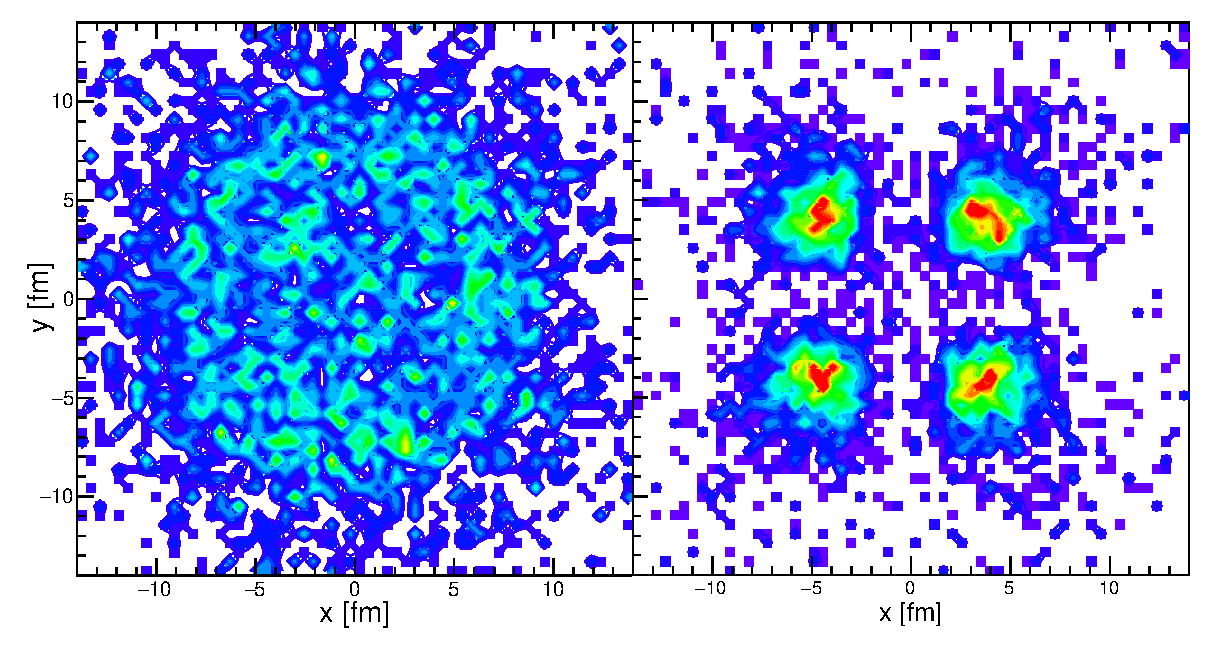
\includegraphics[width=\textwidth]{./figure/xy.eps}
  \caption{Left panel is the original string melting AMPT, right panel is the string melting AMPT that introduce local
           parton density fluctuation.}
  \label{fig:Phase}
\end{figure}



\section{Quark Wigner phase-space functions of $\phi$ and $\Omega$}
For the production of hadronic matter in heavy ion collisions, coalesence model can describe it very well. In our study,
we use coalesence model to study the production of $\Omega$ and $\phi$. The probability for producing a cluster, such as
$\Omega$ and $\phi$, is determined by its Wigner phasespace density without taking the binding
energies into account[[[[song]]]]. The multiplicity of a M-hadron cluster in a heavy-ion collision is given by [[[[[song]]]]]
\begin{equation}
  \label{eq:pro}
  N_{M} = G\int{d\boldsymbol{r}_{i_{1}}}d\boldsymbol{q}_{i_{1}}{\dots}d\boldsymbol{r}_{i_{M-1}}d\boldsymbol{q}_{i_{M-1}}
\times
\left<
  \sum_{i_1>i_2>\dots>i_M}\rho_{i}^{W}(\boldsymbol{r}_{i_{1}},\boldsymbol{q}_{i_{1}}\dots\boldsymbol{r}_{i_{M-1}},\boldsymbol{q}_{i_{M-1}})
\right>.
\end{equation}
Where $\boldsymbol{r}_{i_{1}},\dots,\boldsymbol{r}_{i_{M-1}} and \boldsymbol{q}_{i_{1}},\dots,\boldsymbol{q}_{i_{M-1}}$
are the relative coordinates and momenta in the M-hadron rest frame; $\rho_i^W$ is the Wigner phase-space density of the
M-hadron cluster, and
$\left<...\right>$ denotes the event averaging. G stands for the statistical factor for the cluster.
The wave function of quark can be taken as a spherical harmonic oscillator[[[[[[]]]]]],
\begin{equation}
  \label{eq:wave}
  \psi = (3/\pi^{2}b^{4})^{-3/4}exp
  \left(
    -\frac{\rho^{2}+\lambda^{2}}{2b^2}
  \right)
\end{equation}
Therefore, the quark Wigner function of meson can be expressed as
\begin{equation}
  \label{eq:MESON}
  f_{M}(\boldsymbol{\rho},\boldsymbol{k}_{\rho}) = 8g_{M}exp
  \left[
    -\frac{\boldsymbol{\rho}^2}{\sigmaRho}-\boldsymbol{k}_\rho^{2}\sigmaRho
  \right]
\end{equation}
similarly, the quark Wigner function of baryon can be expressed as
\begin{equation}
  \label{eq:BARYON}
  f_{B}(\boldsymbol{\rho},\boldsymbol{\lambda},\boldsymbol{k}_{\rho},\boldsymbol{k}_{\lambda})
= 8^2g_{B}exp
\left[
  -\frac{\boldsymbol{\rho}^2}{\sigmaRho}-\frac{\boldsymbol{\lambda}^2}{\sigmaLambda}-\boldsymbol{k}_{\rho}^{2}\sigmaRho-\boldsymbol{k}_{\lambda}^{2}\sigmaLambda
\right]
\end{equation}
In Eq (\ref{eq:MESON}) and (\ref{eq:BARYON}),


\section{RESULT}
In this section, we show the results about transverse momentum spectrum and elliptic flows. In Eq (\ref{eq:MESON} and
\ref{eq:BARYON}), The two parameters $\sigma{_{\phi}}$ and $\sigma{_{\Omega}}$ in the quark Wigner phasespace functions
inside the $\phi$ meson and $\Omega$ baryon are related to their root-mean-square radius. For the root-mean-square
radius of hadron, we set the root-mean-square of $\Omega$ is 1.2 fm and $\phi$ is 0.65 fm[[[[[chenliewen]]]]], use these
radius we can study the transverse-momentum spectra of $\Phi$ meson and $\Omega$ baryon as well as their anisotropic
flow in heavy ion collisions.
\subsection{Transverse momentum spectrum}
\begin{figure}[!ht]
  \centering
  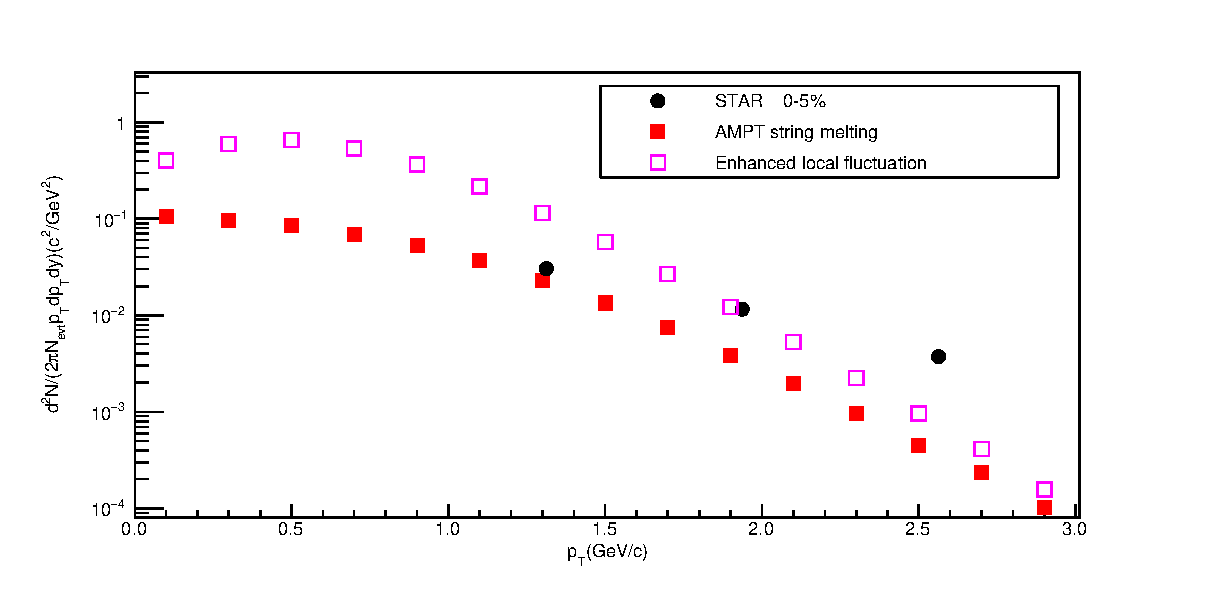
\includegraphics[width=\textwidth]{./figure/omegaYield.eps}
  \caption{omegaYield}
  \label{fig:OmegaYield}
\end{figure}
\begin{figure}[!ht]
  \centering
  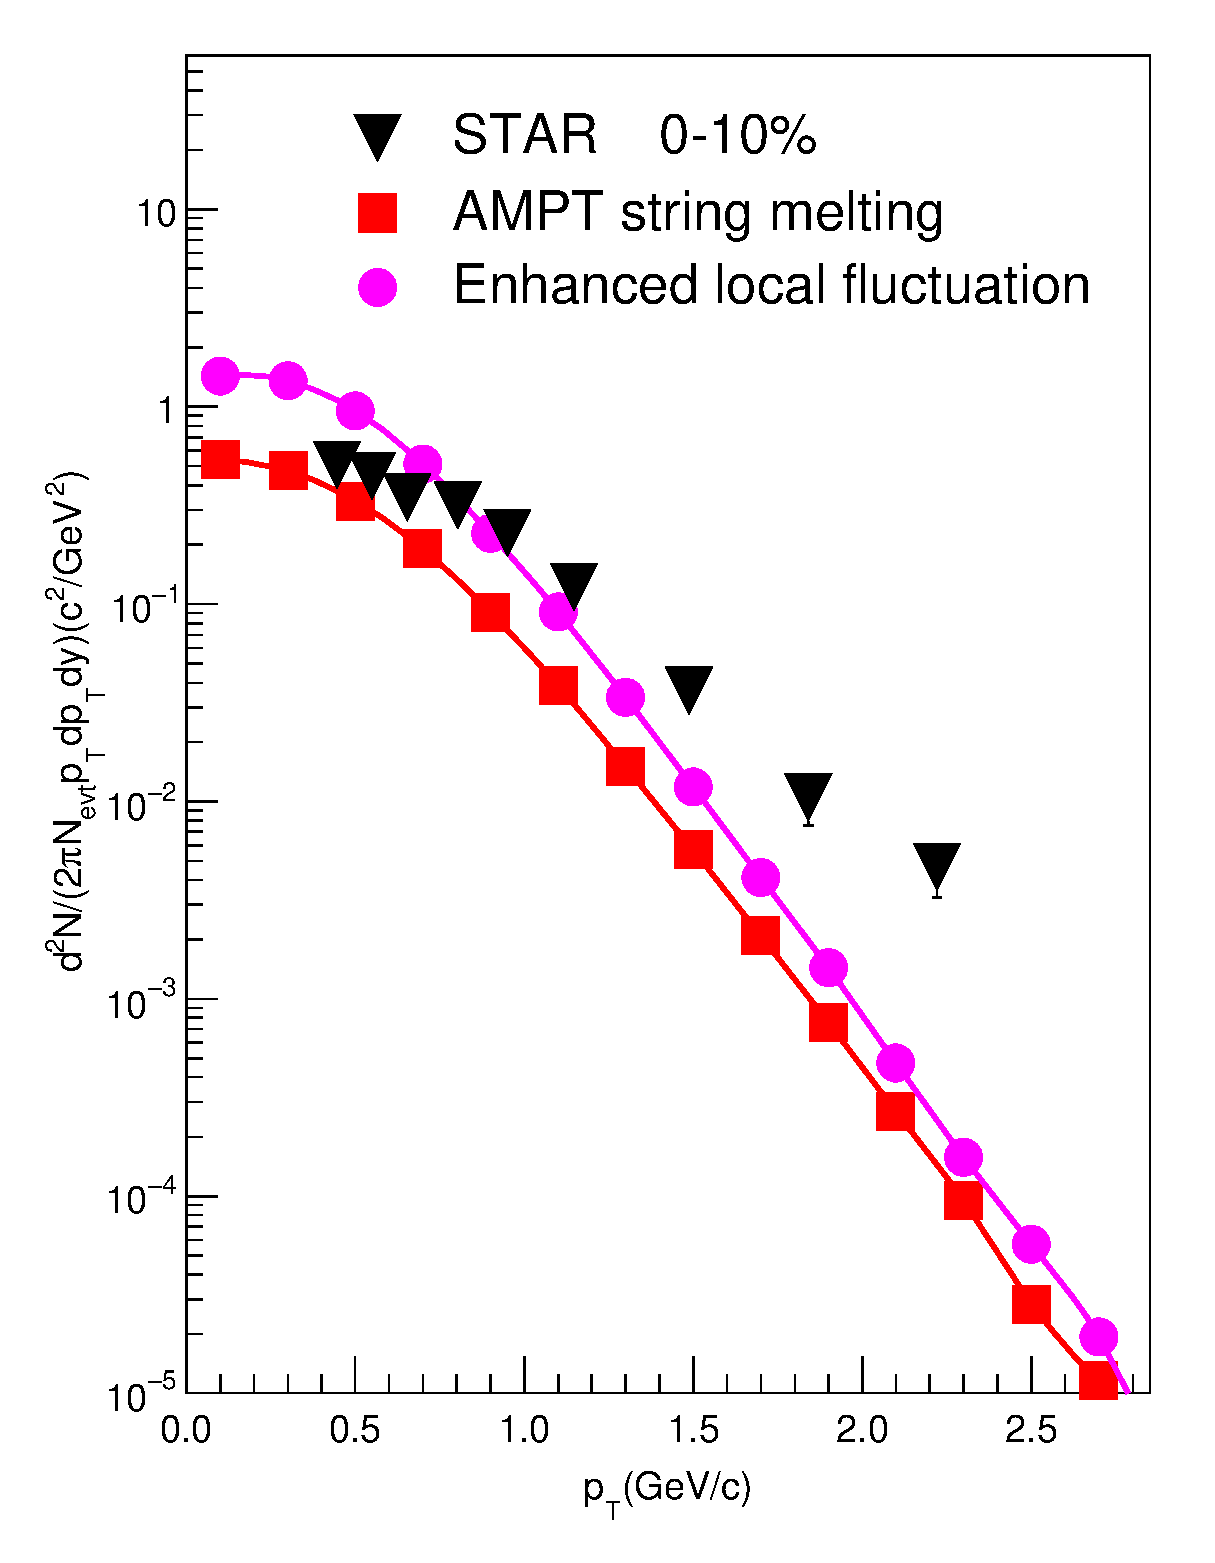
\includegraphics[width=\textwidth]{./figure/phiYield.eps}
  \caption{phiYield}
  \label{fig:PhiYield}
\end{figure}





\end{document}

%%% Local Variables:
%%% mode: latex
%%% TeX-master: t
%%% End:
